\documentclass[ignorenonframetext,]{beamer}
\setbeamertemplate{caption}[numbered]
\setbeamertemplate{caption label separator}{: }
\setbeamercolor{caption name}{fg=normal text.fg}
\beamertemplatenavigationsymbolsempty
\usepackage{lmodern}
\usepackage{amssymb,amsmath}
\usepackage{ifxetex,ifluatex}
\usepackage{fixltx2e} % provides \textsubscript
\ifnum 0\ifxetex 1\fi\ifluatex 1\fi=0 % if pdftex
  \usepackage[T1]{fontenc}
  \usepackage[utf8]{inputenc}
\else % if luatex or xelatex
  \ifxetex
    \usepackage{mathspec}
  \else
    \usepackage{fontspec}
  \fi
  \defaultfontfeatures{Ligatures=TeX,Scale=MatchLowercase}
\fi
% use upquote if available, for straight quotes in verbatim environments
\IfFileExists{upquote.sty}{\usepackage{upquote}}{}
% use microtype if available
\IfFileExists{microtype.sty}{%
\usepackage{microtype}
\UseMicrotypeSet[protrusion]{basicmath} % disable protrusion for tt fonts
}{}
\newif\ifbibliography
\hypersetup{
            pdftitle={Survival analysis in decision modeling},
            pdfauthor={petros.pechlivanoglou@sickkids.ca},
            pdfborder={0 0 0},
            breaklinks=true}
\urlstyle{same}  % don't use monospace font for urls
\usepackage{graphicx,grffile}
\makeatletter
\def\maxwidth{\ifdim\Gin@nat@width>\linewidth\linewidth\else\Gin@nat@width\fi}
\def\maxheight{\ifdim\Gin@nat@height>\textheight0.8\textheight\else\Gin@nat@height\fi}
\makeatother
% Scale images if necessary, so that they will not overflow the page
% margins by default, and it is still possible to overwrite the defaults
% using explicit options in \includegraphics[width, height, ...]{}
\setkeys{Gin}{width=\maxwidth,height=\maxheight,keepaspectratio}

% Prevent slide breaks in the middle of a paragraph:
\widowpenalties 1 10000
\raggedbottom

\AtBeginPart{
  \let\insertpartnumber\relax
  \let\partname\relax
  \frame{\partpage}
}
\AtBeginSection{
  \ifbibliography
  \else
    \let\insertsectionnumber\relax
    \let\sectionname\relax
    \frame{\sectionpage}
  \fi
}
\AtBeginSubsection{
  \let\insertsubsectionnumber\relax
  \let\subsectionname\relax
  \frame{\subsectionpage}
}

\setlength{\parindent}{0pt}
\setlength{\parskip}{6pt plus 2pt minus 1pt}
\setlength{\emergencystretch}{3em}  % prevent overfull lines
\providecommand{\tightlist}{%
  \setlength{\itemsep}{0pt}\setlength{\parskip}{0pt}}
\setcounter{secnumdepth}{0}

\title{Survival analysis in decision modeling}
\subtitle{The DARTH Workgroup}
\author{\href{mailto:petros.pechlivanoglou@sickkids.ca}{\nolinkurl{petros.pechlivanoglou@sickkids.ca}}}
\date{}

\begin{document}
\frame{\titlepage}

\begin{frame}

\end{frame}

\begin{frame}{Partitioned survival models}

\begin{itemize}
\tightlist
\item
  Form of a decision model that:
\item
  Considers evidence of (usually) OS and PFS
\item
  allocates the cohort across pre-progression, post-progression, death
\item
  PFS and OS are modeled independently
\end{itemize}

\end{frame}

\begin{frame}

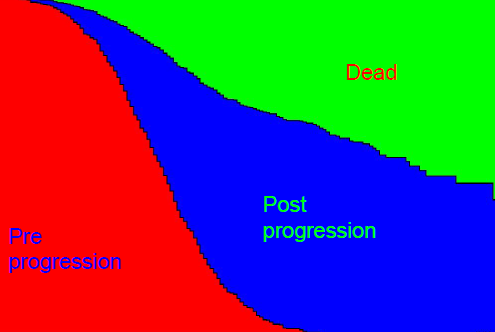
\includegraphics[width=1\linewidth]{figures/psm}

\end{frame}

\begin{frame}{Partitioned survival models}

\begin{itemize}
\item
  Mechanics:
\item
  Remain pre-progression: p(PFS)
\item
  Remain dead: 1 -- p(OS)
\item
  Progressed: p(OS) - p(PFS)
\item
  Implicit assumption: risk of dying is only a function of time
\end{itemize}

\end{frame}

\begin{frame}

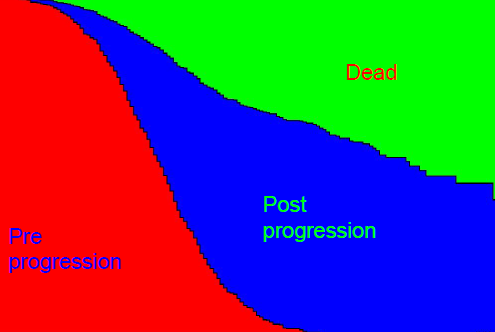
\includegraphics[width=1\linewidth]{figures/psm}

Less problematic with less censoring

\end{frame}

\begin{frame}{Partitioned survival models - the updside}

\begin{itemize}
\tightlist
\item
  Intuitively appealing
\item
  Easy to communicate
\item
  Easy to construct
\item
  In-sync with what is commonly reported in RCTs
\item
  Can be constructed using aggregate / graphic based data
\item
  In-sync with methods of cross-over
\item
  PSMs work great for cases where the whole cohort is observed until
  event of interest (unlikely in the vast majority of the cases)
\end{itemize}

\end{frame}

\begin{frame}{Partitioned survival models - the downside}

\begin{itemize}
\tightlist
\item
  OS and PFS are falsely assumed independent
\item
  Cohort cannot transition back to a healthier state.
\item
  3-state PSM cannot distinguish the origin of the cohort moving to the
  dead state (progresed -\textgreater{} death vs preprogession
  -\textgreater{} death)
\item
  In the presence of censoring:
\item
  Projected trajectory of state occupancy after end of follow up only
  informed by the observed trajectory
\item
  Poor performance when trends in the within trial period may not
  continue in the extrapolation period
\end{itemize}

\end{frame}

\begin{frame}{Partitioned survival models - the criticism}

Woods et al 2017 (DSU 19)


\includegraphics[width=1\linewidth]{figures/psmcritic}

\end{frame}

\begin{frame}

Williams et al 2017 (MDM)

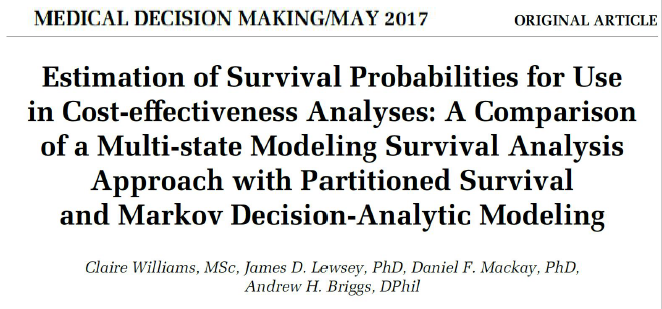
\includegraphics[width=1\linewidth]{figures/williams2017}

\end{frame}

\begin{frame}{Competing Risks}

\begin{itemize}
\tightlist
\item
  Underlying assumption in survival analysis:

  \begin{itemize}
  \tightlist
  \item
    If we could follow censored individuals long enough they would
    experience the event of interest.
  \end{itemize}
\item
  Event B (progression) affecs population size at risk for the competing
  event C
\end{itemize}

\end{frame}

\begin{frame}

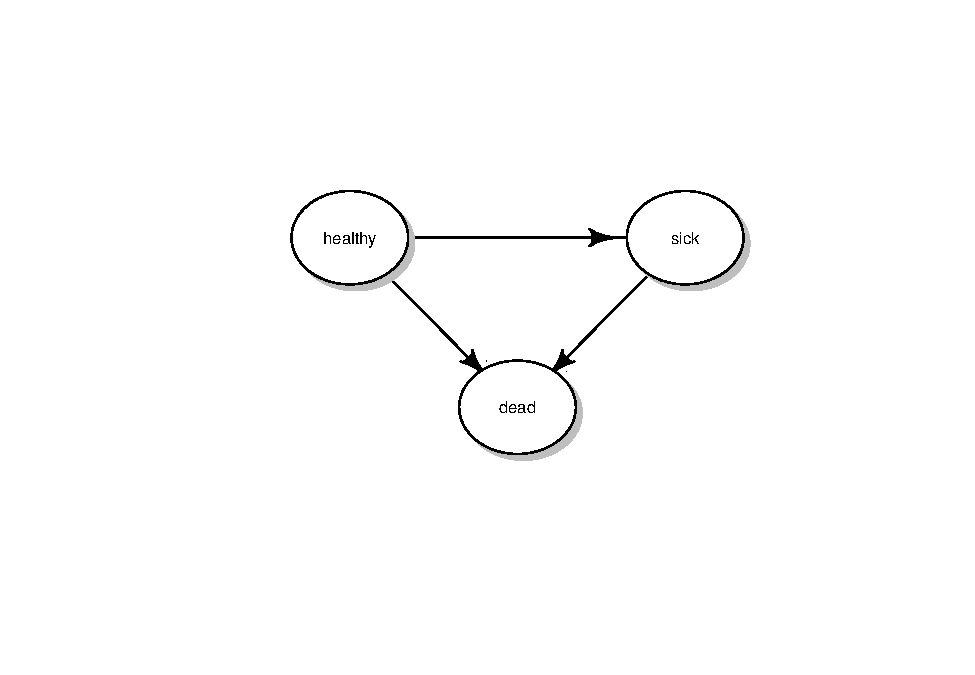
\includegraphics{SMDM_surv_files/figure-beamer/unnamed-chunk-5-1.pdf}

\end{frame}

\begin{frame}{Multistate modeling}

\begin{itemize}
\tightlist
\item
  Extended form of competing risks
\item
  Multivariate survival analysis
\end{itemize}

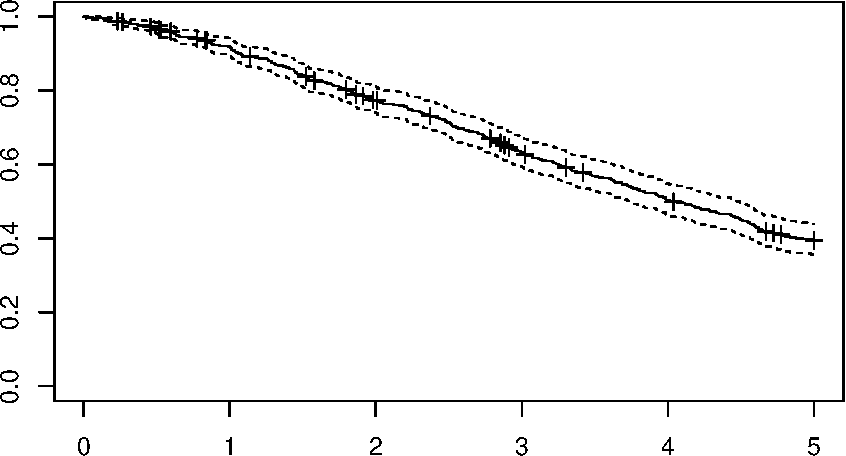
\includegraphics{SMDM_surv_files/figure-beamer/unnamed-chunk-6-1.pdf}

\end{frame}

\begin{frame}{Multistate modeling}

\begin{itemize}
\item
  Extended form of competing risks
\item
  Multivariate survival analysis
\item
  Can incorporate:
\item
  Transition specific covariates
\item
  Recurrent events
\item
  Can work with
\item
  Patient-level data (best)
\item
  Digitized / interval censored data (\ldots{}not best)
\end{itemize}

\end{frame}

\end{document}
